
%%%%%%%%%%%%%%%%%%%%%%% file typeinst.tex %%%%%%%%%%%%%%%%%%%%%%%%%
%
% This is the LaTeX source for the instructions to authors using
% the LaTeX document class 'llncs.cls' for contributions to
% the Lecture Notes in Computer Sciences series.
% http://www.springer.com/lncs       Springer Heidelberg 2006/05/04
%
% It may be used as a template for your own input - copy it
% to a new file with a new name and use it as the basis
% for your article.
%
% NB: the document class 'llncs' has its own and detailed documentation, see
% ftp://ftp.springer.de/data/pubftp/pub/tex/latex/llncs/latex2e/llncsdoc.pdf
%
%%%%%%%%%%%%%%%%%%%%%%%%%%%%%%%%%%%%%%%%%%%%%%%%%%%%%%%%%%%%%%%%%%%


\documentclass[runningheads,a4paper]{llncs}

\usepackage{amssymb}
\setcounter{tocdepth}{3}
\usepackage{graphicx}

\usepackage{url}
\urldef{\mailsa}\path|{alfred.hofmann, ursula.barth, ingrid.haas, frank.holzwarth,|
\urldef{\mailsb}\path|anna.kramer, leonie.kunz, christine.reiss, nicole.sator,|
\urldef{\mailsc}\path|erika.siebert-cole, peter.strasser, lncs}@springer.com|    
\newcommand{\keywords}[1]{\par\addvspace\baselineskip
\noindent\keywordname\enspace\ignorespaces#1}

\usepackage{graphicx,times,amsmath, fontenc}
\usepackage{amssymb}
\usepackage{amsmath}
\usepackage{comment}

\newcommand{\bigO}{\mathcal{O}}
\newcommand{\astar}{\textit{A}$^*$ }
\newcommand{\ambush}{\textit{A}$^*$\textit{mbush}}
\newcommand{\pambush}{\textit{P-A}$^*$\textit{ambush}}
\newcommand{\rambush}{\textit{R-}A$^*$\textit{ambush}}
\newcommand{\sarambush}{\textit{SAR-}A$^*$\textit{ambush}}

\begin{document}

\mainmatter  % start of an individual contribution

% first the title is needed
\title{\ \\ \LARGE\bf A*mbush family: A* Variations for Ambush Behaviour
And Path Diversity Generation}

% a short form should be given in case it is too long for the running head
\titlerunning{Lecture Notes in Computer Science: Authors' Instructions}

% the name(s) of the author(s) follow(s) next
%
% NB: Chinese authors should write their first names(s) in front of
% their surnames. This ensures that the names appear correctly in
% the running heads and the author index.
%

\author{Kelwin Fern\'{a}ndez\and Glebys Gonz\'{a}lez \and Carolina Chang}
%
\authorrunning{Lecture Notes in Computer Science: Authors' Instructions}
% (feature abused for this document to repeat the title also on left hand pages)

% the affiliations are given next; don't give your e-mail address
% unless you accept that it will be published
\institute{Grupo de Inteligencia Artificial,\\
Universidad Sim\'on Bol\'ivar, Venezuela\\
kelwin@gia.usb.ve, glebys@gia.usb.ve, cchang@ldc.usb.ve\\
\url{http://www.gia.usb.ve}}

%
% NB: a more complex sample for affiliations and the mapping to the
% corresponding authors can be found in the file "llncs.dem"
% (search for the string "\mainmatter" where a contribution starts).
% "llncs.dem" accompanies the document class "llncs.cls".
%

\toctitle{Lecture Notes in Computer Science}
\tocauthor{Authors' Instructions}
\maketitle


\begin{abstract}
In the area of Artificial Intelligence for Videogames,
A* is a commonly proposed algorithm  for path-finding. 
Even though this algorithm guaranties optimality, it tends
to bring forth similar behaviours in agents that are
close to each other. On the other hand, when the agents
are sparsely distributed, the algorithm doesn’t secure an
attack that comes from different places. Having the
generation of ambush behaviours and diversity of paths
as the goal, A*mbush, P-A*mbush, R-A*mbush and SAR-A*mbush
are proposed. 
They are modification of A* that considers
the amount of agents that have a specific node
(or edge) in their calculated path, when it’s
computing the cost function of that point in
the graph. P-A*mbush, R-A*mbush and SAR-A*mbush
are variations of A*mbush which tries to improve
the paths generated by the proposed A*mbush algorithm.

\emph{abstract} environment.
\keywords{ambush, pathfinding, A*, group strategies}
\end{abstract}

\section{Introducci\'on}

En el \'area de Inteligencia Artificial para Videojuegos, la generaci\'on
de conductas inteligentes ha sido un reto constante \cite{MF09}, frecuentemente
derivado en el desarrollo de acciones prestablecidas que el usuario puede
f\'acilmente identificar despu\'es de varias ejecuciones del juego.
Esta caracter\'istica es a\'un m\'as com\'un cuando se trata de la generaci\'on
de movimientos t\'acticos y estrat\'egicos grupales, los cuales suelen ser sumamente
complejos de implementar.

Un problema muy tratado en la literatura es la b\'usqueda de caminos
a un punto com\'un, por parte de grupos de agentes dentro de un juego
\cite{MF09}. Este punto suele venir dado por un lugar en el mapa de juego,
potencialmente la posici\'on del oponente. El esquema regularmente utilizado
es generar caminos de costo m\'inimo \cite{HNR72} \cite{RN93}
hacia este punto, sobre el grafo inducido por el mapa del juego. Es
muy probable, que estos caminos confluyan, evitando la diversidad de
rutas y exploraci\'on del mapa.

Al efectuar una persecuci\'on al oponente, la utilizaci\'on de caminos
\'optimos como estrategia deja muchos espacios de escapatoria libres,
por lo que es de especial inter\'es generar mecanismos de diversificaci\'on de
rutas que generen situaciones de emboscada.

\textbf{
En este punto hablar de nuestra soluci\'on y de como esta prob\'o ser
correcta. Mencionar que este art\'iculo pretende ser un soporte adicional
a los dos anteriores para demostrar la validez de las distintas variantes
de forma exhaustiva as\'i como tambi\'en de presentar una nueva m\'etrica
que permite medir de forma m\'as refinada el grado de emboscada.
}

\begin{comment}
La t\'ecnica expuesta pr\'oximamente es adaptable a muchos contextos en
los que, si bien no es necesaria una situaci\'on de emboscada, es
importante generar diversidad de caminos con el fin de no sobresaturar
ciertos sectores del grafo subyacente. Ejemplo de estos son controladores
de tr\'afico, enrutamiento de paquetes f\'isicos o digitales \cite{TMSV03},
rob\'otica, entre otros.
\end{comment}
\begin{minipage}{0.3\textwidth}

\section*{Formal Problem Definition}
\begin{itemize}
\item Let $G = (V,E)$ be a \textbf{graph} (directed or undirected).

\item Let $A$ be a \textbf{set of agents} that want to reach a point
$t \in V$. Every agent $i \in A$, is located in a node of the
graph. Let $pos(i)$ be the position of the agent $i$.

\item A function over $i$ is defined for  determining the
\textbf{cost} of the displacement of the agents  through the graph
$\lambda_i : E \longrightarrow \mathbb{R}^{\geq 0}$.

\item Let $path(i)$ having $i \in A$, be the \textbf{path} that the 
agent $i$ is taking to reach node $t$.

\item The \textbf{degree of ambush} towards the node $t$ is defined as:\\

$\Phi(t) = \dfrac{|\{ i : path(j) = <pos(j),\ \ldots,\ i,\ t>, j \in A\}|}
{\min(|\{ <i,t> : <i,t> \in E \} |,|A|) }$

\end{itemize}
\end{minipage}
\section{Related Works}
A similar problem to the one exposed in this paper is
given by \textit{Space-Time A$^*$} \cite{art3}. In this article, 
a variation of \astar is proposed. It works with an undirected
graph, induced from a grid shaped map. The cost function is common
for all agents and constant between every node pair. 

The main goal of the mentioned paper is to avoid having two 
different agents in the same node at a given instant of time.
For this variation of $A^*$, an expansion in the number of dimensions
of \astar	 is proposed: besides the positions of the agents, the elapsed
time is also taken into account. Thus, \textit{Space-Time A$^*$} has a 
considerable increment in the time and memory costs, because the size
of the search space has grown. 

Other ways of achieving ambush are explained in \cite{art5}. 
This work takes the problem of an agent that has to choose
a path across a rectangle, treated as a grid, and a second 
agent that will have to choose a sub-set of the rectangle trying
to block the path of the first one. The approach in this paper
is to create a matrix of probabilities that evaluates all the
possible combinations of paths and ambush sets, and then
choose the best strategy for both agents through the minimax
algorithm.

\cite{art6} and \cite{art7} approach the previous problem with
sets of continuous nature. In the first work, discrete versions of 
the game model are proposed. Afterwards they are
used to find optimal solutions that satisfy the original
continuous model. The work in \cite{art7} proposes various sets
of solutions for conditions that were not considered in \cite{art6}.

Previous works show exponential search spaces, deriving
in high computational costs. The $A^*mbush$ family is proposed
as an effective method with lower computational order, that can
be used in more general conditions.
\section{A*}

The \astar algorithm \cite{art2,book4,book3} is a variation
of Dijkstra's algorithm \cite{book1} that computes 
paths of minimal cost.
It is an informed search algorithm \cite{book4}, based on 
the following elements:

\begin{itemize}
\item $g$: Represents the accumulated cost from the initial node to the actual node $v$.
\item $\hat{h}$: Is an estimate of the cost from the actual node $v$ to the goal.
\item $\hat{f} = g + \hat{h}$: An estimate of the cost from the initial node to the goal, having $v$ in the path..
\end{itemize}

For the sake of securing optimality, the $\hat{h}$ heuristic 
must be admissible, that is, it shouldn't overestimate any 
cost against the optimal solution.
This algorithm works in a greedy fashion, expanding the next unexplored 
node with the smallest estimated cost $\hat{f}$ at the moment. 
This procedure is repeated until the goal is reached. 

% fin de la nueva def y luego viene lo del orden del algoritmo

The estimated running time of $A^*$ is
$\bigO(|V|log(|V|) + |V|*h + |E|)$.
Having $h$ as the cost of computing function
$\hat{h}$. This cost is derived, assuming an
efficient implementation of the priority queue
such as a Fibonacci heap \cite{book1} and that
the heuristic of each node is only computed
once.
\section{A*mbush}

In this section we propose \ambush, an $A^*$-based
algorithm that solves the ambush generation problem. 
It consists in a modification of $g$ function, that favours
path diversity. We will call this function $g'$.

Let $\Psi(v,i) = 1+(\# j : j \in A \wedge v \in path(j))$,
be the number of agents different from agent $i$, that have the 
node $v$ in their paths towards $t$ plus one. If an agent is not trying to 
reach node $t$ at the moment, or it has not performed the 
search for the node yet, it's path counts as empty. 
Therefore, the agent is not taken into account when calculating
$\Psi(v,i)$'s value. 

It is considered that $g'(pos(i),i) = 0$ for the initial node.
 Let $<v,w>$ be the next edge that should be expanded
from the node $v$, in any of the algorithm's iterations. In
these conditions, the expression that determines $g'$'s value
is $g'(w, i) = g'(v,i) + \lambda_i(<v,w>) \cdot \Psi(w,i)^2$.

Given that $\Psi(v,i) \geq 1$, the path determined by $A^*mbush$
is optimal under the new definition of $g'$. Hence, the properties of
 $A^*$ are preserved \cite{art2}. Nevertheless the path might not 
 be optimal for the original costs function $g$.

Note that $\Psi(v,i) = 1$ for every node $v$ that is not considered
in the path of any agent different to $i$. Similarly,
$\Psi(v,i) > 1$ in any other case. This condition allows the 
agents to consider exploring sub-optimal paths in the 
original graph. The less agents explore this routes, the greater
the chance given to other agents to travel trough them.

\subsection{Complexity}

It is possible to precompute the
function $\Psi$ for node cost's increment. If this function is stored
in a constant structure with fast access, the cost of calculating
$g'$ becomes equal to the cost of computing $g$.
Therefore, the only change if the algorithm's cost
 lays in the initial calculation of function $\Psi$.

The asymptotic complexity of $A^*mbush$ is:
$\bigO(|V|log(|V|) + |V|*h + |E| + |A|*|V| )$.

In the field of video games, the graphs of interest are
given by the polygonal division scheme of the map
\cite{book3,art1} (this polygons tend to have a small
amount of sides), according to the traversable regions 
and their respective adjacencies \cite{book3,art1}. 
Since the number of sides for the polygons is small, this 
graphs tend to have little density. In consequence,
$|E| \in \bigO(|V|)$, this means that the execution 
time of this methods for the graphs of interest in the
area of video games, is considered to be
$\bigO(|V|(log(|V|) + h + |A|) )$. 
The amortized cost of the increment function is $\bigO(|V|)$,
therefore, the amortized cost of the A$^*$mbush algorithm
equals the A$^*$ cost.

\begin{comment}
Figure
\ref{fig:graph_decomp} shows a clear example of a map 
broken into polygons. Each one of them is considered to
be a node in the search space. Two nodes are adjacent if 
their polygons share a common side. 

\begin{figure}[htp]
\centerline{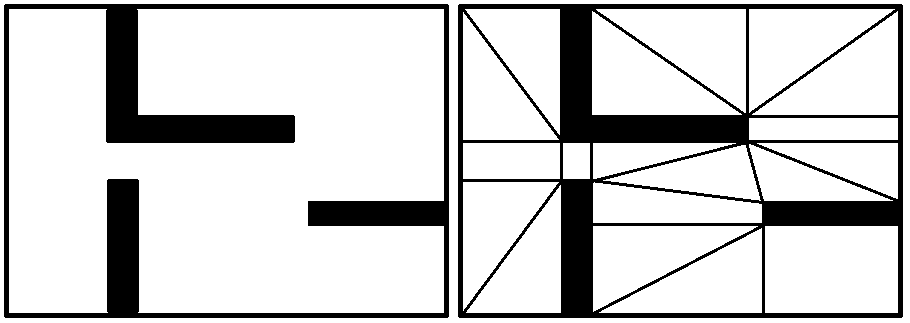
\includegraphics[width=0.6\columnwidth]{figures/graph_decomposition.png}}
\caption{Up: Game map, the black blocks are the obstacles
              Down: Decomposition of the map into convex polygons}
\label{fig:graph_decomp}
\end{figure}
\end{comment}


\section{ P-A*mbush: Ambush with Priorities assignment method P}

Without a strategy that decides which agent calculates it's path 
first, routes that are inconvenient could be chosen, because the 
algorithm doesn't take in account the agent's state in the game. 
For example, if agent $i$ is the closest one to the goal, it could 
be beneficial to make $i$ perform the path computing first. 
This way the agent won't end up tacking a long route to generate 
ambush, wasting an opportunity to catch the wanted element,
 while an agent that was further away takes the most direct way.
 
 For this work two a simple P method is proposed based on 
 the real distance between the agents an the goal. This is
 because the positions of the agents are a very general and
 intuitive property that defines the advantage that an element
 could have over another.
 Other character properties like strength, remaining
 life, stamina, and any others could be used in this method to 
 generate the desired group strategy while performing \ambush.
 
 Figure \ref{fig:grids} shows the path that three agents would take when 
 performing \ambush\ (left Image) and \pambush\ with
 real distance (right Image).
 The circles represent the agents, the numbers inside them represent the order
 in which each agent computes the path it will take and the black cross represents
 the goal.
 
 \begin{figure}[htp]
\centerline{
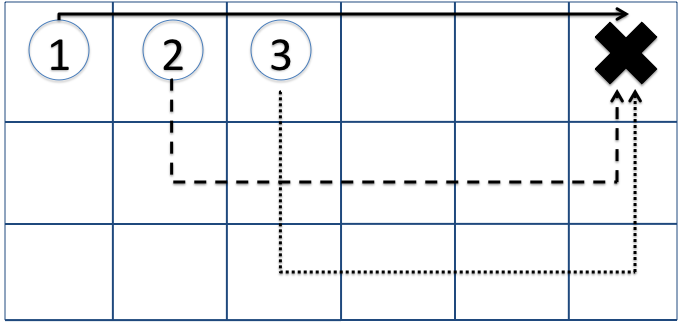
\includegraphics[width=0.4\columnwidth]{figures/ambush_grid.png}
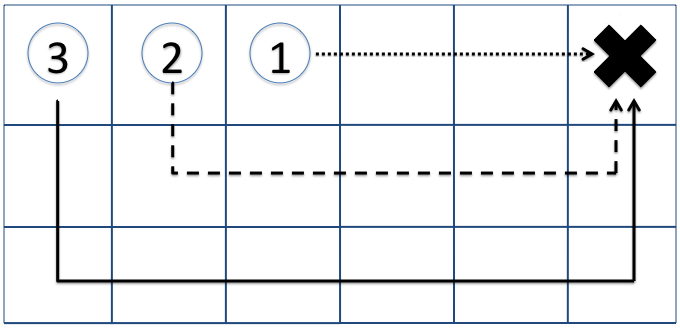
\includegraphics[width=0.4\columnwidth]{figures/priorities_grid.png}
}
\caption{The numbers represent the order in which the agents
are calculating the path.
Up: Performance of \ambush. Since it does not take the distance to the
              goal into account, the agent that is closer to the goal, takes a longer path.
              Down: Performance of \pambush\ using $A^*$'s distance. The agent that
              can reach the goal first using the path given by \astar has the top priority for
              calculating the path, the second closest by this distance goes afterwards, and so on.}
\label{fig:grids}
\end{figure}

When using \pambush, the behaviours of the agents look more intelligent, 
since the one that is closer to the goal is taking the most direct path to reach it, instead
of the circling around like the one performing \ambush\ does.

Other advantage that \pambush\ displays is that  the
goal will always be reached in the minimum time possible by 
one of the agents. Thus,  this algorithm shows qualitative
improvements over  \ambush.

Although the cost of computing \pambush\ with real distance is
bigger than computing \ambush\ for one agent, the amortized
cost invested to calculate \pambush\ for each agent equals
\ambush's amortized cost.
However, having agents perform \textit{P-A}$^*$\textit{mbush} with real distance 
would decrease the frame rate because of the involved constants.
Therefore, using the euclidean 
distance is proposed as a good middle. It will not perform as well as 
the one using $A^*$'s distance, but also, it's computational cost will
not differ from the one in \ambush.
\section{ R-A*mbush: Ambush with fixed radio R}

Getting agents to perform \ambush\ from the starting 
point can be disadvantageous, since they can take 
unnecessarily longer routes, when avoiding each other’s paths. 
Making the agents perform \ambush\ when they are closer
 to the goal could shorten the increment in this cost. 
 
With this reasoning as a base, \rambush\ is proposed.
 It is an A$^*$mbush modification that performs \astar until
the agent gets inside a fixed radius $R$ around the goal point.
Once at this stage, the agent stats performing \ambush. 
Note that this transition happens only once. Even if  the
\ambush\ algorithm makes the agent leave the radio area,
it will not start performing \astar again. This prevents a 
loop that the intelligence could easily fall into. First, the agent,
following the path given by A$^*$ comes inside the radius R,
then \ambush\ takes it out of the area when trying to go for 
a unexplored route, subsequently, this behaviour is interrupted 
and the A$^*$ method takes control again, making the agent go 
inside the radio. Those steps could be repeated infinitely, 
so once the radio $R$ is crossed, only \ambush\ behaviour takes place.
Figure \ref{fig:rambush} shows the performance of the \rambush\
algorithm.

\begin{figure}[htb]
	\centerline{
		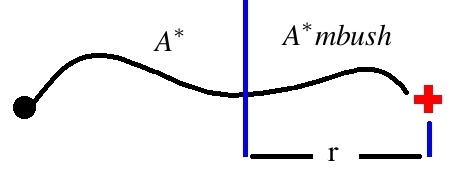
\includegraphics[width=0.48\columnwidth]{figures/rambush.jpg}
	}
	\caption{\label{fig:rambush}
	     R-A$^*$mbush. The agent located in the black point
	     tries to reach the cross.}
\end{figure}

The radius $R$ is measured in real distance (A$^*$). 
It was chosen over the Euclidean, because obstacles in games 
could make the agents take ambush routes when the path to 
get to the goal is still very long, and this would antagonize 
the purpose of reducing the path cost when possible.

\section{ Self Adaptive R-A*mbush: Ambush with adaptive radius R}

\rambush\  provides a solution that is not as general as the one for
 \ambush.  Using the same distance $R$ for the fixed radius 
 in different maps, would produce good results in some of them 
 and bad ones in others. This means the user would have to manually 
 fix the measure of $R$ by tacking into consideration the size of 
 the map, the path cost function, or the number of obstacles. 
 In addition, given that  the cost function can be different for each 
 agent, the radius should be established according to the 
 $\lambda$ measure of every agent.
  
Thus, \sarambush\ is proposed as a variation of \rambush\ that 
solves this generality problem. Initially, This method makes each
 agent calculate the path with \astar. Then, a set of points from
  that route is chosen.  This will  be the set of the possible radius 
  $R$. The algorithm will select the minimum radius that generates 
  the greatest $\Phi$, starting from the smallest $R$.  
  This is based on the idea of starting to use sub-optimal 
  paths as late as possible.  Note that \astar\ is the specific 
  case where $R=0$ and \ambush\ is the one where $R$ is greater 
  than or equal to the real distance between the agent and the goal.  

If points that are too close to the goal are inside the set of radius, 
in particular, $R=0$, all the other agents will choose the optimal path, 
once the maximum ambush is reached. This could make the 
distribution of the agents around the goal very unbalanced towards 
the nodes that are closest to the agents stating points.

Figure \ref{unbalanced} Shows a situation where the agents distribution 
is not desirable, but the maximum ambush rate is obtained.	The agents 
colored in black performed the method \sarambush\ first. Then, the agents
in gray chose the optimal path because the ambush measure cannot 
be improved anymore, creating an unbalanced distribution around the
goal. This can be solved by taking into account a measure
 of distribution when choosing the radius. Thus, let 

\begin{equation}
  \Delta = 1-\dfrac{(\Sigma i |  i \in V 
  						\wedge i \in pred(t)
  						\wedge num(i) > 
  							\left\lceil \frac{n}{|pred(t)|} \right\rceil 
  					:  num(i) - 
  						\left\lceil \frac{n}{|pred(t)|} \right\rceil}		
  						{n-\left\lfloor \frac{n}{|pred(t)|} \right\rfloor}
\end{equation}

\noindent
be a metric related with the rate of agents that need to
reach the goal from another node to have them equally
distributed. The value of the metric is 1 when the
agents are perfectly distributed and it tends to zero
when the agents are unbalanced.
In the formula, $n$ represents the number of agents that
already calculated the path.  $pred(t)$  is the set of nodes adjacent to
the goal node. Finally $num(i)$ is the number of agents that reached 
the target from the node $i$. 
The numerator of the main fraction counts the number of the agents
that need to be swapped and the denominator is the number of
swaps in the worst case scenario (all agents reaching the goal
from one node). The only purpose of the subtraction is to
use the lexicographical order in the objective function of
the strategy.
For example, for Figure \ref{unbalanced} $\Delta = 0.66$.
This means that equal distribution can be reached by making one of
the agents that are on the node at the left of the goal, ambush it
from above.

\begin{figure}[htb]
	\centerline{
		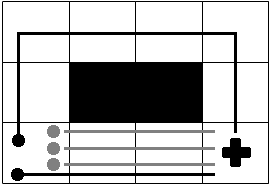
\includegraphics[width=0.48\columnwidth]{figures/unbalanced.png}
	}
	\caption{\label{unbalanced}
	     Unbalanced ambush.}
\end{figure}

The algorithm would search for the maximum ambush
rate and in case of a tie it would go for the path that
achieves the best distribution. The $\Delta$ value alone is
not enough to compare two ambush strategies.

\subsection{Complexity}

This variation of \ambush\ is more inefficient than the
original version. If $T(G,A)$ is the
complexity in time of computing \ambush\ for a graph
$G=(V,E)$ with $|A|$ agents and the number of candidates 
to be selected as radius points is $k$, the complexity
of the \sarambush\ is $\bigO(k\cdot T(G,A))$.

Since $k \in \bigO(V)$ (selecting every possible node
as radius) the worst case of the algorithm is
$\bigO(|V|\cdot T(G,A))$. Alternative candidate sets
can be constructed from taking nodes that are separated
by distances that are incremented exponentially, for
example, selecting the nodes in positions that are
powers of two in the \astar\ path ($1, 2, 4, 8, \ldots$).
This variation leads to an increment of only $\bigO(log(|V|))$.
In the following experiments the radius set contains
every node in the \astar\ path.

\section{Experimentos}
\label{sec:experiments}

Para cada experimento se estudian cinco algoritmos:
una implementaci\'on base de \astar que sirve de referencia,
una implementaci\'on de caminos simples aleatorios mediante
b\'usqueda en profundidad, \ambush, \pambush con mecanismo
de prioridad determinado por la distancia real de los agentes
a la meta y finalmente, \sarambush.

presentan resultados del incremento medio porcentual de los caminos.
Para cada topolog\'ia de grafo, se generan aleatoriamente 100 grafos,
sobre los cuales se ejecutan experimentos con 100 disposiciones distintas
de agentes y del nodo objetivo.
Para cada uno de estos algoritmos se muestra el valor de emboscada
utilizando la m\'etrica originalmente propuesta y utilizando la
m\'etrica propuesta en el presente trabajo. El n\'umero de agentes
es variado con el fin de mostrar su impacto en el grado de emboscada
y en el incremento derivado de la escogencia de caminos sub\'optimos.
Adem\'as se muestran resultados con las dos instancias de mapas ($g1$ y $g2$)
presentadas en el trabajo previo \cite{FGC12} con 60 y 85 nodos
respectivamente. Estos mapas provienen de la poligonalizaci\'on del mapa
de juego en pol\'igonos. Estas restricciones son ampliamente utilizadas
en juegos\cite{MF09}. Estos grafos se pueden visualizar en la figura \ref{fig:gs}.

\begin{figure}[htb]
	\begin{center}
		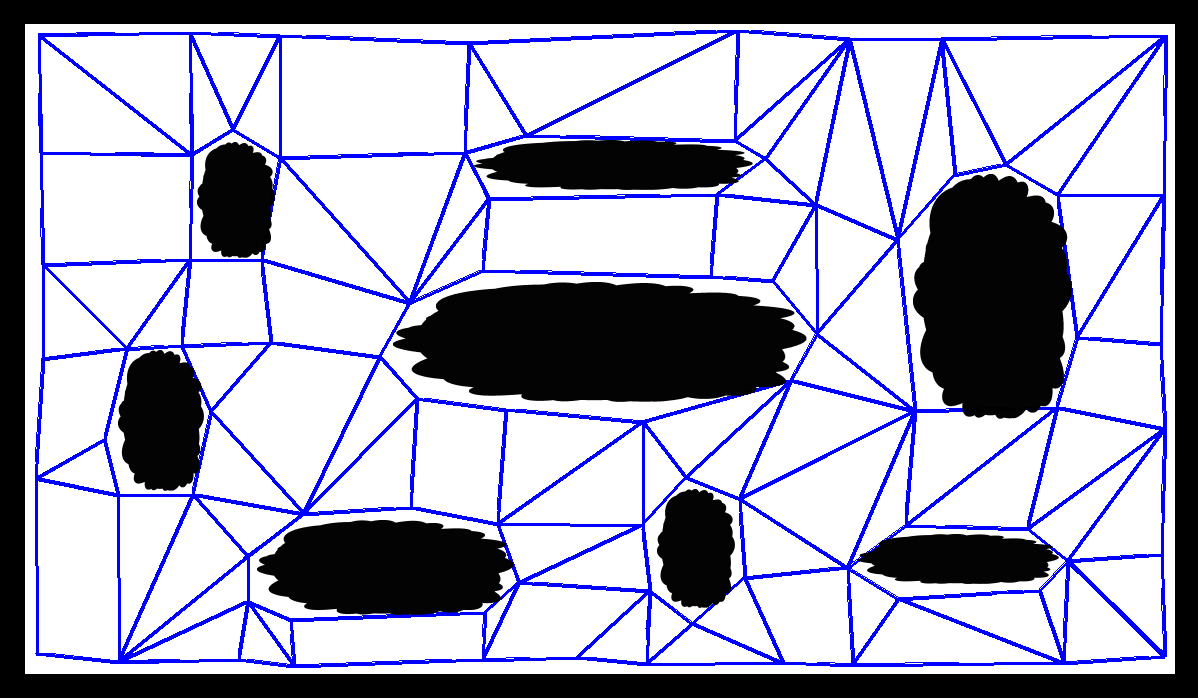
\includegraphics[scale=0.23]{figures/g1.png}
		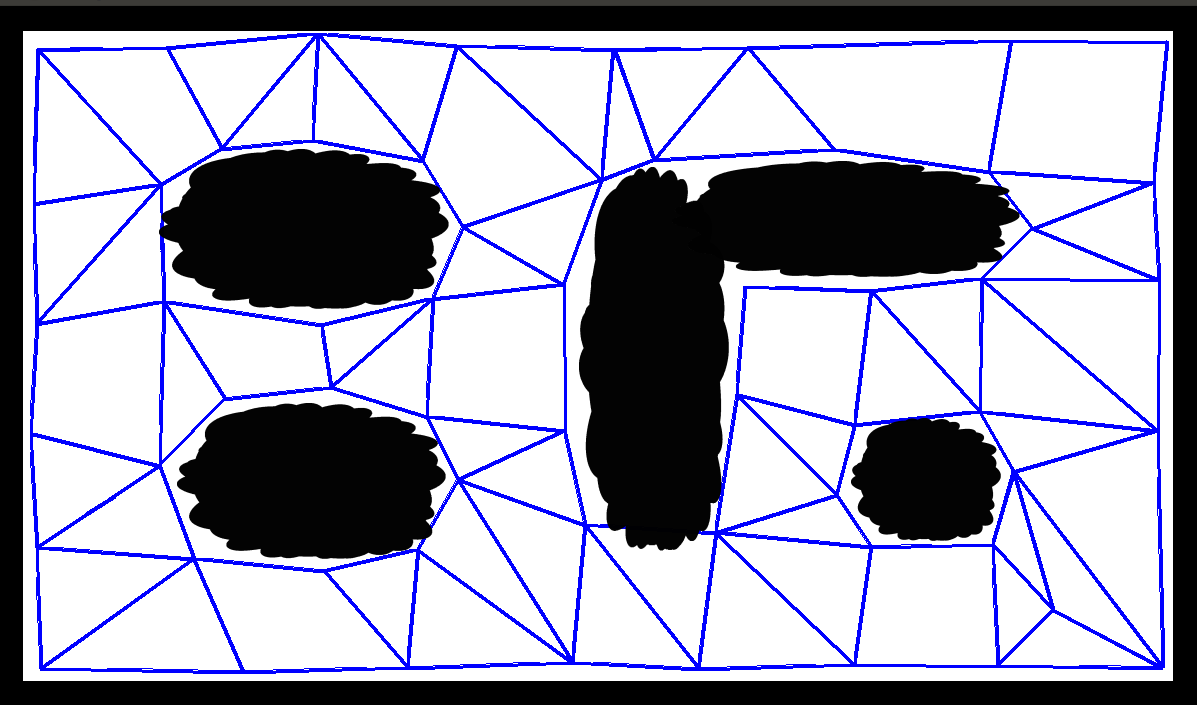
\includegraphics[scale=0.23]{figures/g2.png}
	\end{center}
	\caption{\label{fig:gs}
	     \textbf{Arriba:} Mapa 1 poligonalizado (60 pol\'igonos).
	     \textbf{Abajo:} Mapa 2 poligonalizado (85 pol\'igonos).
     }
\end{figure}

\section{Conclusions}

With a raise in the computational cost that has little significance,
$A^*mbush$ generates an evident upgrade in the ambush behavior.
Likewise, $P$-$A^*mbush$ shows a superior behavior over the traditional
$A^*mbush$, because it successfully increases the path diversity.


As it can be appreciated in the results, even in the worst case scenario, 
the $A^*mbush$ family never produces a result that is worse than the one made
by $A^*$. On the same line, $P$-$A^*mbush$ does not show in any
case a downgrade when compared with $A^*mbush$. 

$SAR$-$A^*mbush$ always shows the smallest incremental distance. And the
best ambush rates when the maps are large. Although, due it's computational
cost, the use of $P$-$A^*mbush$ could be more desirable when the
 processing resources are limited.

When paths are diverse, the agents performing any of the $A^*mbush$ 
methods become more naturally distributed over the map. 
Not having all the elements rounded up in a small space
can be advantageous when agents change from
one state of behavior to another. For example, if the conduct changes 
from pursue to flee, the ambush based algorithms not only allow a
better behavior, but also, they maintain the agents further away from each
other, which is a better disposition when it comes to strategies of scape.

In contrast with the pre-established conducts that are generally implemented 
for acting up in specific situations or moments of each game, the
proposed algorithms enhance the diversity of ambush situations that
can be produced as a tactical move from the agents. 

$P$-$A^*mbush$ generates an upgrade to the way the intelligence 
in the agent's behavior is perceived and $SAR$-$A^*mbush$ delivers an
even better looking one. This way, not only the paths become 
more variate, but the conduct of the agents looks better.
It makes the elements in the game act in a way that looks more
natural and perform an ambush strategy that is more effective.

For more results and experiments visit  http://www.gia.usb.ve/~kelwin/ambush/.
  
%\section{Future Works}


Given the nature of the algorithm, it is possible for agents to
take paths that are long at some points when it is not needed. 
The possibility of a selective incorporation of the algorithm will
be explored. This strategy would have the goal of making the
 incremental distance as minimal as possible.

Likewise, the inclusion of a maximum capacity for nodes or edges
will be studied. This variation corresponds to the problem proposed in
\cite{art3}, when all the edges have an unitary capacity. 

Additionally, an heuristic will be implemented to restrict the 
ambush behaviour to a radius around the goal. This way, 
both path and computational costs could be reduced. 
This heuristic can also be adapted to generate several levels
of game difficulty.


  

\begin{thebibliography}{4}

\bibitem{book1}
T.~Cormen, C.~Leiserson, R.~Rivest and C. Stein, \emph{Introduction to Algorithms, 3rd ed}.\hskip 1em plus 0.5em minus 0.4em\relax
  The MIT Press, 2009.
  
\bibitem{book2}
M.~Gendreau and J.~Potvin, \emph{Handbook of Metaheuristics, 2nd ed}.\hskip 1em plus 0.5em minus 0.4em\relax
  Springer, 2010.  

\bibitem{book3}
I.~Millington and J.~Funge, \emph{Artificial Intelligence for Games, 2nd ed}.\hskip 1em plus 0.5em minus 0.4em\relax
  Morgan Kaufmann Publishers, 2009.  

\bibitem{book4}
S.~Russell and P.~Norvig, \emph{Artificial Intelligence: A Modern Approach, 2nd ed}.\hskip 1em plus 0.5em minus 0.4em\relax
  	Prentice-Hall, Englewood Cliffs, NJ,, 1993.  
  
\bibitem{art1}
X.~Cui and H.~Shii, ``Direction oriented pathfinding in video games,'' \emph{International Journal of Artificial Intelligence  \& applications 2}, 2011.

\bibitem{art2}
P.~Hart, N.~Nilsson and B.~Raphael, ``Correction to “a formal basis for the heuristic determination of minimum cost paths”,'' \emph{SIGART Newsletter 37}, pp. 28--29, 1972.

\bibitem{art3}
D.~Silver, ``Cooperative pathfinding,'' \emph{ AI Game Programming Wisdom 3}, pp. 99--111, 2006.

\bibitem{art4}
R.~Teixeira, K.~Marzullo, S.~Savaje and G.~Voelker, ``In search of path diversity in isp networks,'' \emph{ IMC}, pp. 27--29, 2003.

\bibitem{art5}
W.~Ruckle, R.~Fennell, P.~Holmes and C.~Fennemore, ``Ambushing Random Walks I: Finite Models,'' \emph{Operations Research, vol 24}, No. 2, 1976.

\bibitem{art6}
W.~Ruckle, ``Ambushing Random Walks II: Continuous Models,'' \emph{Operations Research, vol 29}, No. 1, 1981.

\bibitem{art7}
I.~Woodward, ``Discretization of the Continuous Ambush Game,'' \emph{Naval Research Logistics, Vol. 50}, 2003.

\bibitem{web1}
E.~Haines, ``Point in Polygon Strategies,''
\emph{http://erich.realtimerendering.com/ ptinpoly/}, 2001.

\end{thebibliography}

\end{document}
